\documentclass{exam}
\usepackage[utf8]{inputenc}
\usepackage{lmodern}
\usepackage{microtype}

% \usepackage[parfill]{parskip}
\usepackage[dvipsnames]{xcolor}
\usepackage{amsmath}
\usepackage{amsfonts}
\usepackage{amsthm}
\usepackage{siunitx}
\DeclareSIUnit\year{yr}
\DeclareSIUnit\foot{ft}
\DeclareSIUnit\litre{\liter}

\usepackage{skull}

\usepackage{pgfplots}
\usepgfplotslibrary{polar}
\pgfplotsset{compat=1.11}
\usepackage{graphicx}
\usepackage{sidecap}
\sidecaptionvpos{figure}{c}
\usepackage{float}
\usepackage{gensymb}
\usepackage{tkz-euclide}
\usetkzobj{all}
\usepackage{commath}
\usepackage{hyperref}
\usepackage{enumitem}
\usepackage{wasysym}
\usepackage{multicol}
\usepackage{mathtools}
\usepackage{tcolorbox}
\usepackage{tabularx}
\usepackage[version=4]{mhchem}
\usepackage{changepage}
\usepackage{listings}
\lstset{basicstyle=\ttfamily\linespread{0.8}\small}

\renewcommand*{\thefootnote}{\fnsymbol{footnote}}

\newtheorem*{thm}{Theorem}
\newtheorem*{iden}{Identity}
\newtheorem*{lemma}{Lemma}
\newtheorem{obs}{Observation}
\theoremstyle{definition}
\newtheorem*{defn}{Definition}
\newtheorem*{ex}{Example}
\newtheorem{con}{Construction}
\newtheorem*{alg}{Algorithm}

\newtheoremstyle{break}
  {\topsep}{\topsep}%
  {\itshape}{}%
  {\bfseries}{}%
  {\newline}{}%
\theoremstyle{break}
\newtheorem*{bthm}{Theorem}

% russian integral
\usepackage{scalerel}
\DeclareMathOperator*{\rint}{\scalerel*{\rotatebox{17}{$\!\int\!$}}{\int}}

% \DeclareMathOperator*{\rint}{\int}

\pgfplotsset{vasymptote/.style={
    before end axis/.append code={
        \draw[densely dashed] ({rel axis cs:0,0} -| {axis cs:#1,0})
        -- ({rel axis cs:0,1} -| {axis cs:#1,0});
    }
}}

% \pointsinrightmargin
\boxedpoints
\pointname{}

\newcommand{\questioA}{\question[\texttt{\textbf{\color{Cerulean} A}}]}
\newcommand{\questioM}{\question[\texttt{\textbf{\color{PineGreen} M}}]}
\newcommand{\questioE}{\question[\texttt{\textbf{\color{WildStrawberry} E}}]}
\newcommand{\questioS}{\question[\texttt{\textbf{\color{Goldenrod} S}}]}
\newcommand{\questioO}{\question[\texttt{\textbf{\color{BurntOrange} O}}]}

\newcommand{\parA}{\part[\texttt{\textbf{\color{Cerulean} A}}]}
\newcommand{\parM}{\part[\texttt{\textbf{\color{PineGreen} M}}]}
\newcommand{\parE}{\part[\texttt{\textbf{\color{WildStrawberry} E}}]}
\newcommand{\parS}{\part[\texttt{\textbf{\color{Goldenrod} S}}]}
\newcommand{\parO}{\part[\texttt{\textbf{\color{BurntOrange} O}}]}

\newcommand{\subparA}{\subpart[\texttt{\textbf{\color{Cerulean} A}}]}
\newcommand{\subparM}{\subpart[\texttt{\textbf{\color{PineGreen} M}}]}
\newcommand{\subparE}{\subpart[\texttt{\textbf{\color{WildStrawberry} E}}]}
\newcommand{\subparS}{\subpart[\texttt{\textbf{\color{Goldenrod} S}}]}
\newcommand{\subparO}{\subpart[\texttt{\textbf{\color{BurntOrange} O}}]}

\newcommand{\mainHeader}[2]{\section*{NCEA Level 2 Mathematics\\#1. #2}}
\newcommand{\mainHeaderHw}[2]{\section*{NCEA Level 2 Mathematics (Homework)\\#1. #2}}


\begin{document}

\mainHeader{11}{Slopes and Differentiation}
The main theme this year so far has been geometry and modelling the real world. This week, we move from modelling the stationary world
of fields, fences, and compound interest to the world of continuity and motion.

We have already seen that if we model a changing quantity with a linear equation of the form $ y = mx + c $, then it is possible to
talk about the rate of change of that quantity by means of the slope of the graph of the equation.

\begin{ex}
  Suppose that the amount of sand in a pile (in kilograms, perhaps) is modelled by the equation $ \text{mass} = 3(\text{time}) + 1 $.
  Then the slope of the graph of mass versus time is 3, and so it makes sense to say that the rate of change of mass is three kilograms
  per unit of time.
\end{ex}

Our goal this week is to describe the slopes of functions which are not necessarily lines. Let us look at some arbitrary function $ f $,
and let us draw the graph $ y = f(x) $. Then, recalling that we originally defined slope to be $ m = \frac{\text{change in } y}{\text{change in } x} $,
we can look at the slope between $ y_0 = f(x_0) $ and $ y_1 = f(x_1) $:
\begin{center}
\fbox{\begin{tikzpicture}
  \begin{axis}[
    axis lines = none,
    xlabel = $ x $,
    ylabel = {$ y = f(x) $}
  ]
    \addplot[domain = -3:5, color = black, samples = 100] {(x + 1)*(x - 2)*(x - 3) + 2};
    \node[label={right:{$\left(x_0,f(x_0)\right)$}},circle,fill,inner sep=2pt] at (axis cs:-2,-18) {};
    \node[label={left:{$\left(x_1,f(x_1)\right)$}},circle,fill,inner sep=2pt] at (axis cs:4,12) {};
    \draw[style=dotted] (-2,-18) -- (4,12);
  \end{axis}
\end{tikzpicture}}
\end{center}
The average slope betwen $ (x_0, f(x_0)) $ and $ (x_1, f(x_1)) $ is just the slope of the dotted line, which is simply
\begin{displaymath}
  \frac{\text{rise}}{\text{run}} = \frac{y_1 - y_0}{x_1 - x_0} = \frac{f(x_1) - f(x_0)}{x_1 - x_0}.
\end{displaymath}
If we move the point $ (x_0, y_0) $ closer to $ (x_1, y_1) $ along the curve, then it makes sense that the slope of the dotted line will
match the slope of $ y = f(x) $ at the point $ (x_1, y_1) $ better and better (the dotted lines in the diagram below). If we imagine moving
the point $ (x_0, y_0 ) $ until it coincides with the point $ (x_1, y_1) $, then the `average' slope (indicated by the solid line below) will
in face be the actual slope of the curve at $ x_1 $.
\begin{center}
\fbox{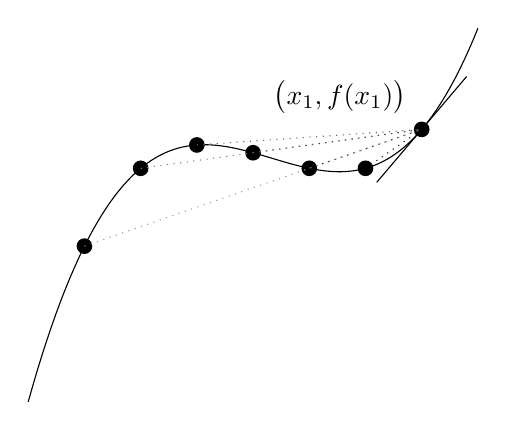
\begin{tikzpicture}
  \begin{axis}[
    axis lines = none,
    xlabel = $ x $,
    ylabel = {$ y = f(x) $}
  ] %(x -2)(x - 3) + (x + 1)(x - 3) + (x + 1)(x - 2) = x^2 - 5x + 6 + x^2 - 2x - 3 + x^2 - x - 2 = 3*16 - 2*16 + 1
    \addplot[domain = -3:5, color = black, samples = 100] {(x + 1)*(x - 2)*(x - 3) + 2};
    \node[circle,fill,inner sep=2pt] at (axis cs:-2,-18) {};
    \node[circle,fill,inner sep=2pt] at (axis cs:-1,2) {};
    \node[circle,fill,inner sep=2pt] at (axis cs:0,8) {};
    \node[circle,fill,inner sep=2pt] at (axis cs:1,6) {};
    \node[circle,fill,inner sep=2pt] at (axis cs:2,2) {};
    \node[circle,fill,inner sep=2pt] at (axis cs:3,2) {};
    \node[label={above left:{$\left(x_1,f(x_1)\right)$}},circle,fill,inner sep=2pt] at (axis cs:4,12) {};
    \draw[color=black!40, style=dotted] (-2,-18) -- (4,12);
    \draw[color=black!50, style=dotted] (-1,2) -- (4,12);
    \draw[color=black!60, style=dotted] (0,8) -- (4,12);
    \draw[color=black!70, style=dotted] (1,6) -- (4,12);
    \draw[color=black!80, style=dotted] (2,2) -- (4,12);
    \draw[color=black!90, style=dotted] (3,2) -- (4,12);
    \addplot[domain = 3.2:4.8, color=black]{12 + (x - 4)*17};
  \end{axis}
\end{tikzpicture}}
\end{center}

\begin{ex}
  Suppose we look at the curve $ y = x^2 $. The two points $ (0,0) $ and $ (2,4) $ are on this curve; the average slope
  of the curve between $ x= 0 $ and $ x = 2 $ is therefore $ \frac{4 - 0}{2 - 0} = 2 $.

  Now, suppose we want to find the actual slope of the parabola at $ x = 2 $. We will do this in a slightly tricky way:
  finding the average slope between $ x = 2 $ and $ x = 2 + h $, and then setting $ h $ to zero. The coordinates of the
  point on the parabola at $ x = 2 + h $ will be $ (2 + h, (2 + h)^2) = (2 + h, 4 + 4h + h^2) $ and so the average slope
  that we are looking for is
  \begin{displaymath}
    \frac{\text{rise}}{\text{run}} = \frac{(4 + 4h + h^2) - 4}{(2 + h) - 2} = \frac{4h + h^2}{h} = 4 + h;
  \end{displaymath}
  hence the average slope between $ x = 2 $ and $ x = 2 + h $ when $ h = 0 $ (i.e. when the two points are the same),
  and thus the actual slope of $ y = x^2 $ at $ x = 2 $, is 4.

  More generally, suppose we are to find the slope of the parabola at $ (x_0, x_0^2) $. To do this, we will find
  the average slope between this point and the point $ (x_0 + h, (x_0 + h)^2) = (x_0 + h, x_0^2 + 2x_0 h + h^2) $.
  The calculation runs as follows:
  \begin{displaymath}
    \frac{\text{rise}}{\text{run}} = \frac{(x_0^2 + 2x_0 h + h^2) - x_0^2}{(x_0 + h) - x_0} = \frac{2x_0 h + h^2}{h} = 2x_0.
  \end{displaymath}

  Does this function give us the slope we expect? For $ x < 0 $, the parabola is downward-sloping (if we move to the right,
  we move down) and so we would expect the slope to be negative; and for $ x > 0 $, the parabola is upwards-sloping and
  so we would expect the slope to be positive. The function $ x \mapsto 2x $ satisfies both these criteria, and so this is
  reassuring: our algebraic slope-finding seems to have given a reasonable answer.

  Hence, given the function $ f : x \mapsto x^2 $, we can write down another function $ f' : x \mapsto 2x $ that gives the
  slope of the graph $ y = f(x) $ at any point we choose.
\end{ex}

It is, in fact, possible with most functions $ f $ we have met to write down another function $ f' $ such that the second
function (called the \emph{derivative} of $ f $) gives the slope of $ y = f(x) $ at any point we choose.

\begin{ex}
  Let's try $ f(x) = x^3 $ now; we'll go a bit quicker this time.
  \begin{displaymath}
    \frac{\text{rise}}{\text{run}} = \frac{(x + h)^3 - x^3}{(x + h) - h} = \frac{x^3 + 3x^2h + 3xh^2 + h^3 - x^3}{h}
                                                                         = 3x^2 + 3xh + h^2
  \end{displaymath}
  and so (setting $ h $ to zero) it seems that the derivative of $ f $ is $ f' : x \mapsto 3x^2 $.

  Does this make sense? Well, $ y = x^3 $ is always sloping upwards, and $ 3x^2 $ is never negative, so yes --- this
  does make sense.
\end{ex}

With the basic examples out of the way, I will state (without proof, but the proof is similar to the ideas above) the following
theorem.
\begin{thm}[Power rule]
  If $ f $ is a function defined by $ f(x) = ax^r $, where $ r $ is any real number, then the derivative of $ f $ is the function
  defined by $ f'(x) = rax^{r - 1} $.
\end{thm}

This matches our example above: for $ x^2 $, we obtained $ 2x = 2x^{2 - 1} $ and for $ x^3 $ we obtained $ 3x^2 = 3x^{3 - 1} $. Note
though that this theorem holds when $ r $ is any real number. Hence:

\begin{ex}\leavevmode
  \begin{enumerate}
    \item The derivative of $ 3x^{2018} $ is $ 6054x^{2017} $.
    \item The derivative of $ 9x^\pi $ is $ 9\pi x^{\pi - 1} $.
    \item The derivative of $ 97 $ is $ 0 $.
    \item The derivative of $ \sqrt{x} $ is $ \frac{1}{2}x^{-1/2} $.
    \item The derivative of $ 1/x $ is $ -\frac{1}{x^2} $.
  \end{enumerate}
\end{ex}

\clearpage
We also have the following theorem which allows us to combine derivatives:

\begin{thm}
  If $ f $ and $ g $ are functions, and $ \lambda $ is any number, then
  \begin{enumerate}
    \item $ (\lambda)' = 0 $ --- the derivative of a flat line/constant is zero.
    \item $ (f + g)' = f' + g' $ --- the derivative of the sum of two functions is the sum of the derivatives.
    \item $ (\lambda f)' = \lambda f' $  --- the derivative of a number times a function is the number times the derivative.
  \end{enumerate}
\end{thm}

Hence,
\begin{ex}\leavevmode
  \begin{enumerate}
    \item The derivative of $ 2x^2 + 3x $ is $ 4x + 3 $.
    \item The derivative of $ 19x^{\sqrt{2}} - 3 $ is $ 19\sqrt{2}x^{\sqrt{2} - 1} $.
  \end{enumerate}
\end{ex}

Finally, we can obviously take derivatives with respect to variables that are not $ x $;
obviously the two functions $ x \mapsto f(x) $ and $ y \mapsto f(y) $ are the same function,
and the derivative of $ 3y^2 $ with respect to $ y $ is $ 6y $.

If we want to make the variable of differentiation clear, we can use the alternative Leibniz
notation: if $ y = f(x) $, then the derivative is
\begin{displaymath}
  \text{either} \qquad f' \qquad\text{ or }\qquad \od{y}{x}.
\end{displaymath}

If we take the derivative of the derivative, the result is called the second derivative and
is notated by
\begin{displaymath}
  \text{either} \qquad f'' \qquad\text{ or }\qquad \od[2]{y}{x}.
\end{displaymath}

In general, the $n$th derivative is notated by
\begin{displaymath}
  \text{either} \qquad f^{(n)} \qquad\text{ or }\qquad \od[n]{y}{x}.
\end{displaymath}
I am aware that the notation $ f^{(n)} $ is awful as it looks like an exponent, and so never will
never use it myself.

\clearpage
\subsection*{Questions}
\begin{questions}
  \question Since the sum rule for derivatives holds (i.e. $ (f + g)' = f' + g' $), one might be tempted
            to guess that the product rule $ (fg)' = f'g' $ also holds. Unfortunately, this is not the case.
    \begin{parts}
      \part Differentiate $ f(x) = 4x^3 $, $ g(x) = 2x^2 $, and $ h(x) = 8x^5 $.
      \part Notice that $ fg = h $, but $ f' g' \neq h' $.
      \part There is in fact a product rule for derivatives, but this year you won't need it. Find
            the derivative $ \od{y}{x} $ if $ y = (3x + 2)(x^2 + 1) $.
    \end{parts}
  \question Differentiate the function, with respect to $ x $ or the stated variable.
    \begin{parts}
      \part $ a(x) = 186.5 $
      \part $ b(x) = \sqrt{30} $
      \part $ c(x) = 5x - 1 $
      \part $ z = -4x^{10} $
      \part $ e(x) = x^3 - 4x + 6 $
      \part $ f(t) = \frac{1}{2} t^6 - 3t^4 + t $ with respect to $ t $
      \part $ g(x) = x^2 (1-2x) $
      \part $ h(x) = (x - 2)(2x + 3) $
      \part $ y = x^{-2/5} $
      \part $ B(y) = cy^{-6} $ with respect to $ y $
    \end{parts}
  \question The following part-questions require you to find higher derivatives
            of functions.
    \begin{parts}
      \part Find $ \od[2]{x}{t} $ if $ x = 3t^2 + 4 $.
      \part Suppose $ f(x) = 9x^2 + \frac{1}{x^3} + \sqrt{x} $. Find $ f''(x) $.
      \part Find $ \od[3]{y}{t} $ if $ y = 3x^{-1} $.
      \part Find $ f''(x) $ if $ f'(x) = 9x^2 + 3x^{-2} $.
      \part Find $ a(t) = \od[2]{s}{t} $ if $ s(t) = 3t - 4t^{-1} $.
    \end{parts}
  \question If we `zoom out' from the graph of any polynomial, and ignore the `wiggly bits' in the middle, the result
            always `looks like' either the graph of $ y = \pm x^2 $, or the graph of $ y = \pm x^3 $.
    \begin{parts}
      \part Check this by zooming out from $ y = 3x^6 + 2x^3 - 17x^2 + 3 $ and $ y = -2x^9 + 30x^2 - x $ on a graphing calculator.
      \part Intuitively justify why the derivative of an odd polynomial (one which has an odd highest power of $ x $) is an even
            polynomial, and the derivative of an even polynomial is an odd polynomial.
    \end{parts}
  \question Where is the graph of $ y = \frac{x^2}{2} - \frac{x^3}{3} $ increasing?
  \clearpage
  \question Draw the graph of the slope function (derivative) for each of the following graphed functions.
    \begin{parts}
      \part \fbox{\begin{tikzpicture}
              \begin{axis}[
                axis lines = center,
                xlabel = $ x $,
                ylabel = {$ y = f(x) $},
                xmin = -3, xmax = 5,
                ymin = -8, ymax = 40
              ]
                \addplot[domain = -3:5, color = black, samples = 100] {x^2 + 3*x - 3};
              \end{axis}
            \end{tikzpicture}}
            \fbox{\begin{tikzpicture}
              \begin{axis}[
                axis lines = center,
                xmin = -3, xmax = 5,
                ymin = -8, ymax = 40
              ]
%                 \addplot[domain = -3:5, color = black, samples = 100] {x^2 + 3*x - 3};
              \end{axis}
            \end{tikzpicture}}
      \part \fbox{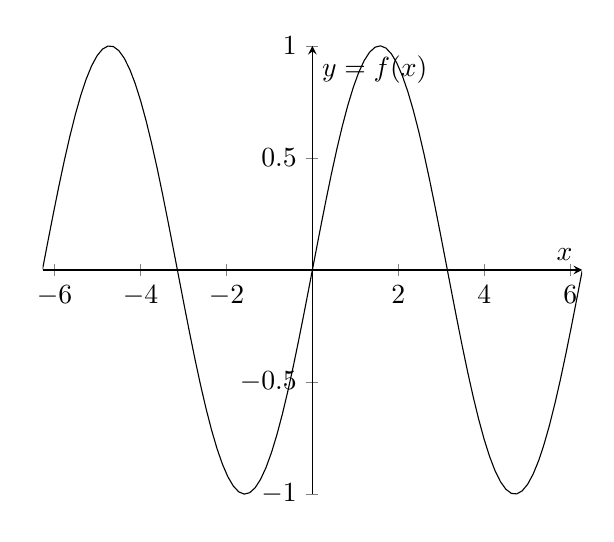
\begin{tikzpicture}
              \begin{axis}[
                axis lines = center,
                xlabel = $ x $,
                ylabel = {$ y = f(x) $},
                xmin = -6.28, xmax = 6.28,
                ymin = -1, ymax = 1
              ]
                \addplot[domain = -6.28:6.28, color = black, samples = 100] {sin(deg(x))};
              \end{axis}
            \end{tikzpicture}}
            \fbox{\begin{tikzpicture}
              \begin{axis}[
                axis lines = center,
                xmin = -6.28, xmax = 6.28,
                ymin = -1, ymax = 1
              ]
%                 \addplot[domain = -6.28:6.28, color = black, samples = 100] {sin(deg(x))};
              \end{axis}
            \end{tikzpicture}}
      \part \fbox{\begin{tikzpicture}
              \begin{axis}[
                axis lines = center,
                xlabel = $ x $,
                ylabel = {$ y = f(x) $},
                xmin = -1, xmax = 5,
                ymin = -15, ymax = 30
              ]
                \addplot[domain = -1:5, color = black] {-(x - 1)*(x - 2)*(x - 4)};
              \end{axis}
            \end{tikzpicture}}
            \fbox{\begin{tikzpicture}
              \begin{axis}[
                axis lines = center,
                xmin = -1, xmax = 5,
                ymin = -40, ymax = 5
              ]
%                 \addplot[domain = -1:5, color = black] {-(x - 1)*(x - 2)*(x - 4)};
              \end{axis}
            \end{tikzpicture}}
      \part \fbox{\begin{tikzpicture}
              \begin{axis}[
                axis lines = center,
                xlabel = $ x $,
                ylabel = {$ y = f(x) $},
                xmin = -1, xmax = 5,
                ymin = -5, ymax = 5
              ]
                \addplot[domain = -1:2, color = black] {2*x - 3};
                \addplot[domain = 2:5, color = black] {0.5*(x-2)^2 + 1};
              \end{axis}
            \end{tikzpicture}}
            \fbox{\begin{tikzpicture}
              \begin{axis}[
                axis lines = center,
                xmin = -1, xmax = 5,
                ymin = -1, ymax = 9
              ]
%                 \addplot[domain = -1:2, color = black] {2*x - 3};
%                 \addplot[domain = 2:5, color = black] {0.5*(x-2)^2 + 1};
              \end{axis}
            \end{tikzpicture}}
      \part \fbox{\begin{tikzpicture}
              \begin{axis}[
                axis lines = center,
                xlabel = $ x $,
                ylabel = {$ y = f(x) $},
                xmin = -5, xmax = 5,
                ymin = -5, ymax = 5
              ]
                \addplot[domain = -5:-0.1, color = black] {1/x};
                \addplot[domain = 0.1:5, color = black] {1/x};
              \end{axis}
            \end{tikzpicture}}
            \fbox{\begin{tikzpicture}
              \begin{axis}[
                axis lines = center,
                xmin = -5, xmax = 5,
                ymin = -5, ymax = 5
              ]
%                 \addplot[domain = -5:0.1, color = black] {1/x};
%                 \addplot[domain = 0.1:5, color = black] {1/x};
              \end{axis}
            \end{tikzpicture}}
    \end{parts}
  \question Car tires need to be inflated properly because overinflation or
            underinflation can cause premature treadwear. The graph shows
            tire life $ L $ (in thousands of kilometres) for a certain type
            of tire at various pressures $ P $ (in kPa), as well as a quadratic
            function that models the tire life.

            \begin{center}
              \fbox{\includegraphics[width=0.5\textwidth]{tires}}
            \end{center}

            Use the model to estimate $ \od{L}{P} $ when $ P = 200 $ and when
            $ P = 300 $. What is the meaning of the derivative? What is the
            significance of the sign of the derivatives?
  \clearpage
  \question A function $ f $ is given by $ f(x) = 2 - 4x + 4x^2 + ax^3 $. The gradient of the graph at the point where $ x = 1 $ is 3. Find
            the value of $ a $.
  \question Let $ f $ be a function of $ x $ defined by $ f(x) = 3x^2 + 6x + 6 $. Show that $ f $ is a solution
            of the \emph{differential equation} $ f(x) - f'(x) = 3x^2 $.
  \question Show that the function $ f $ of $ y $ defined by $ f(y) = \frac{3}{y^2} + 2y $ is not differentiable at $ y = 0 $.
  \question It is natural to ask if there is any function such that the function is
            its own derivative.
    \begin{parts}
      \part An obvious candidate is the function $ K $ defined by $ K(x) = 0 $. Show that $ \od{K}{x} = K(x) $.
      \part For a more interesting example, we will look at the exponential functions $ y = a^x $. Draw the
            gradient function of $ y = 2^x $; explain why looking at the exponential functions is probably a
            productive way to answer our question.
      \part Suppose we try to use the same technique as we used with the parabola. Show that the average slope
            between $ (x, a^x) $ and $ (x + h, a^{x + h}) $ is given by
            \begin{displaymath}
              a^x \left(\frac{a^h - 1}{h}\right).
            \end{displaymath}
      \part For $ a^x $ to be its own slope, we want $ \frac{a^h - 1}{h} $ to get closer and closer to 1 as $ h $ gets
            closer and closer to zero. Unfortunately we can't just substitute $ h = 0 $ straight in. Why?
      \part Let $ a = (1 + h)^{1/h} $ (where we take $ h $ very small), and show that $ \frac{a^h - 1}{h} = 1 $. This
            suggests that $ a $ works as a base for our exponential-which-is-its-own-derivative if we let $ h $ get closer to zero here.
      \part Again, we can't let $ h = 0 $ in $ a $ --- so let $ n = 1/h $, and show that $ a = \left(1 + \frac{1}{n}\right)^n $.
      \part If $ n \to 0 $, then $ h \to \infty $. Therefore, our base we want is just $ \left(1 + \frac{1}{n}\right)^n $ if we
            let $ n $ get infinitely large: the notation we use is
            \begin{displaymath}
              \lim_n \left(1 + \frac{1}{n}\right)^n,
            \end{displaymath}
            which you can read as the \emph{limit} with respect to $ n $. Calculate this base for some large value of $ n $. Is the number you see familiar?
    \end{parts}
\end{questions}

\end{document}
